\documentclass{article}
\usepackage[margin=1in]{geometry}
\usepackage{problemset}

\showsolntrue

% Custom commands
\newcommand{\R}{\mathbb{R}}
\newcommand{\X}{\mathcal{X}}
\newcommand{\Y}{\mathcal{Y}}
\newcommand{\E}{\mathbb{E}}
\newcommand{\V}{\text{Var}}
\renewcommand{\P}{\mathbb{P}}
\newcommand{\x}{\mathbf{x}}
\newcommand{\w}{\mathbf{w}}
\newcommand{\z}{\mathbf{z}}

\begin{document}

\pstitle{%
    COGS 181%
}{
    Homework 4%
}[due Thursday, February 19 at 11:59PM]

\begin{probset}
% --- Problem 1 ---
\begin{prob}[\textbf{(28 points) Conceptual Questions}]
    \begin{subprobset}
    \begin{subprob}
        \textbf{(4 points)} For image recognition problems (e.g. detecting a cat in a photo), which architecture of neural network would be best suited to solve the problem?

        \begin{enumerate}[label=\Alph*.]
            \item 2-layer neural networks.
            \item Convolutional Neural Network (CNN).
            \item 4-layer neural networks.
            \item Perceptron.
        \end{enumerate}

        \begin{soln}
            B. Convolutional Neural Network (CNN).
        \end{soln}
    \end{subprob}

    \begin{subprob}
        \textbf{(4 points)} Which of the following gives non-linearity to a neural network?

        \begin{enumerate}[label=\Alph*.]
            \item Stochastic Gradient Descent (SGD).
            \item Rectified Linear Unit (ReLU).
            \item Convolutional layer (Conv).
            \item Average Pooling layer (AvgPool).
        \end{enumerate}

        \begin{soln}
            B. Rectified Linear Unit (ReLU).
        \end{soln}
    \end{subprob}

    \begin{subprob}
        \textbf{(4 points)} In the figure below, we observe that the error curves (both training and validation) have many “ups and downs”:

        \begin{center}
            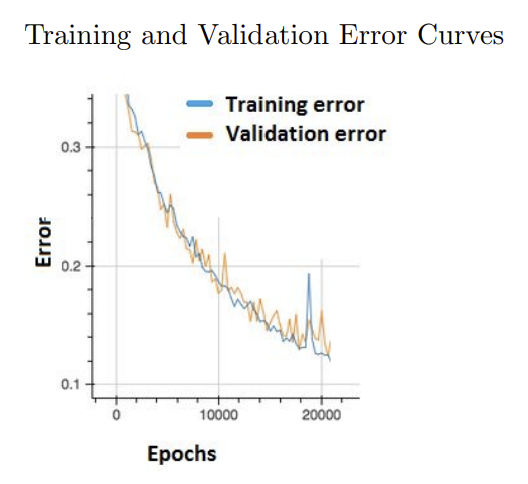
\includegraphics[width=0.3\textwidth]{Images/1.3.png}
        \end{center}

        Should we worry about the training process? Choose the \textbf{best} explanation below:

        \begin{enumerate}[label=\Alph*.]
            \item Yes, because the “ups and downs” means there is a problem with the learning rate of the neural network.
            \item Yes, because the “ups and downs” means there is a problem with the model design of the neural network.
            \item No, as long as there is a cumulative decrease in both training and validation errors, we do not need to worry.
            \item No, since the error is too low ($ < 0.2$ after 10,000 epochs), we do not need to worry about the oscillation of the error.
        \end{enumerate}

        \begin{soln}
            C. No, as long as there is a cumulative decrease in both training and validation errors, we do not need to worry.
        \end{soln}
    \end{subprob}

    \begin{subprob}
        \textbf{(4 points)} Which of the following is \textbf{the most probable} about model capacity (model capacity means the ability of the neural network to approximate complex functions)? 

        \begin{enumerate}[label=\Alph*.]
            \item As the number of data points in a mini-batch increases, model capacity increases.
            \item As the training loss after convergence increases, model capacity increases.
            \item As the learning rate increases, model capacity increases.
            \item As the number of learnable parameters increases, model capacity increases.
        \end{enumerate}

        \begin{soln}
            D. As the number of learnable parameters increases, model capacity increases.
        \end{soln}
    \end{subprob}

    \begin{subprob}
        \textbf{(4 points)} There is a dataset of 28 $\times$ 28 pixel handwritten digits nicely prepared to train a neural network, but we accidentally scrambled the images by re-ordering the pixels in some totally meaningless way, and now we can't get the original dataset back! Below is an image of a handwritten '2' before and after being scrambled.

        \begin{figure}[H]
            \centering
            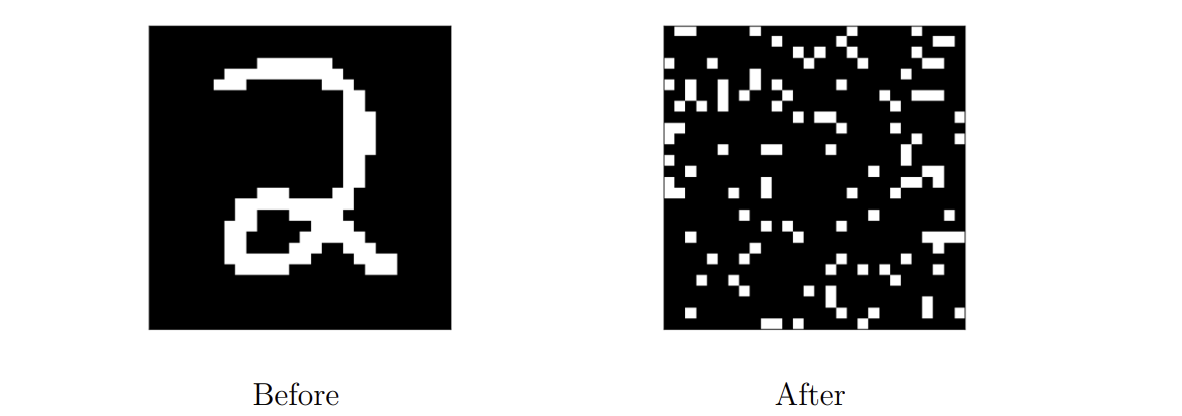
\includegraphics[width=\textwidth]{Images/fig1.png}
            \caption{An image of a handwritten '2' before and after being scrambled.}
        \end{figure}

        Luckily, all of the images (in both the training set and the test set) were changed \textbf{in the same way}. For example, if pixels number 1 and number 3 switched places in one image, then they switched places in every other image as well. Because of that, a student thinks that a neural network can still be successfully trained after all. Whether that student is right or not depends largely on the type of neural network that the student has in mind. Which of the following neural networks will be at a disadvantage because of the mistake? Choose \textbf{all} that apply.

        \begin{enumerate}[label=\Alph*.]
            \item A feed-forward neural network with no hidden layer and no convolution layer.
            \item A convolutional neural network where the size of each weight filter is 8 $\times$ 8 (stride of 1 and no padding).
            \item A convolutional neural network where the size of each weight filter is 28 $\times$ 28 (stride of 1 and no padding).
            \item None of the above.
        \end{enumerate}

        \begin{soln}
            B and C
        \end{soln}
    \end{subprob}

    \begin{subprob}
        \textbf{(4 points)} A Convolutional Neural Network (CNN) has 3 consecutive 5 $\times$ 5 convolutional layers with a stride of 1 without pooling. What is the size of the receptive field for a neuron (the set of input image pixels that activate the neuron) in the 3rd convolutional layer?

        \begin{enumerate}[label=\Alph*.]
            \item 5.
            \item 9.
            \item 13.
            \item 125.
        \end{enumerate}

        \begin{soln}
            C. 13
        \end{soln}
    \end{subprob}

    \begin{subprob}
        \textbf{(4 points)} Choose one that is \textbf{least likely} to help reduce overfitting in neural network:

        \begin{enumerate}[label=\Alph*.]
            \item Dropout
            \item Batch Normalization
            \item Momentum
            \item L2 Regularization
        \end{enumerate}

        \begin{soln}
            C. Momentum
        \end{soln}
    \end{subprob}
    \end{subprobset}
\end{prob}

\newpage

% --- Problem 2 ---
\begin{prob}[\textbf{(15 points) Activation Functions}]
    For each activation on the left-hand side, find and connect the corresponding plot of the activation function on the right-hand side.

    \begin{center}
        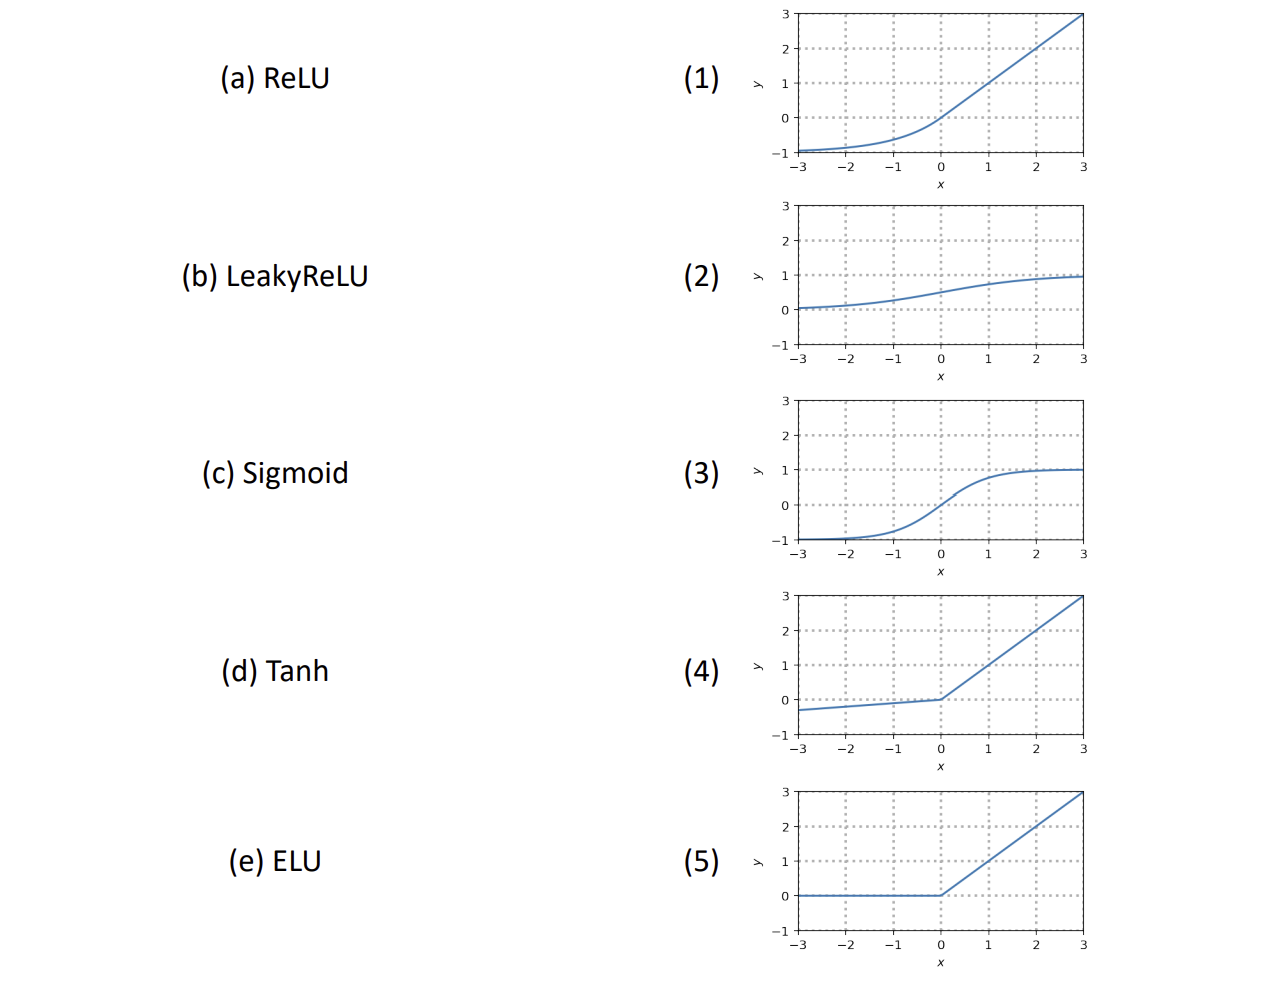
\includegraphics[width=0.9\textwidth]{Images/2.png}
    \end{center}

    \begin{soln}
        a - 5, b - 4, c - 2, d - 3, e - 1
    \end{soln}
\end{prob}

\newpage

% --- Problem 3 ---
\begin{prob}[\textbf{(18 points) Convolution neural networks}]
    The 1D convolution operation (we compute the \textbf{correlation} here actually) is defined as:

    \begin{align}
        h(i) = f(i) \ast g(i) = \sum_{j=-\infty}^{\infty} f(i + j) \times g(j),
    \end{align}

    where $f$ is a 1-dimensional input vector and $g$ is a convolution filter (kernel). $h(i)$ is often called a response map. The Rectified Linear Unit operation on variable $a$ is defined as:

    \begin{align}
        ReLU(a) = \max(0, a).
    \end{align}

    The Max Pooling (window size=2, stride=1) operation on an output map $q(i)$ is defined as:

    \begin{align}
        Max(q, i) = \max(q(i), q(i + 1)).
    \end{align}

    The Average Pooling (window size=2, stride=1) operation on an output map $q(i)$ is defined as:

    \begin{align}
        Avg(q, i) = \frac{q(i) + q(i + 1)}{2}.
    \end{align}

    Given an input data vector $f$:

    \begin{center}
        \begin{tabular}{|c|c|c|c|c|c|}
            \hline
            $i$ & 1 & 2 & 3 & 4 & 5 \\
            \hline
            $f(i)$ & 10 & 50 & 30 & 20 & 10 \\
            \hline
        \end{tabular}
    \end{center}

    The convolution filter (kernel) $g$ is defined as:

    \begin{center}
        \begin{tabular}{|c|c|c|c|}
            \hline
            $i$ & -1 & 0 & 1 \\
            \hline
            $g(i)$ & -2 & 0 & 1 \\
            \hline
        \end{tabular}
    \end{center}

    Please fill the table below, by sequentially implementing operations including: convolution, activation, and pooling. Note that the stride of convolution is 1, $M axP ool(ReLU(h), i)$ and $AvgP ool(ReLU(h), i)$ are \textbf{two alternative operations} that both take in $ReLU(h(i))$.

    \begin{center}
        \begin{tabular}{|c|c|c|c|c|c|c|c|}
            \hline
            $i$ & 0 & 1 & 2 & 3 & 4 & 5 & 6 \\
            \hline
            $f(i)$ & 0 & 10 & 50 & 30 & 20 & 10 & 0 \\
            \hline
            $h(i) = f(i) \ast g(i)$ & gray & 50 & 10 & -80 & -50 & -40 & gray \\
            \hline
            $ReLU(h(i))$ & gray & 50 & 10 & 0 & 0 & 0 & gray \\
            \hline
            $MaxPool(ReLU(h), i)$ & gray & 50 & 10 & 0 & 0 & gray & gray \\
            \hline
            $AvgPool(ReLU(h), i)$ & gray & 30 & 5 & 0 & 0 & gray & gray \\
            \hline
        \end{tabular}
    \end{center}
\end{prob}

\newpage

% --- Problem 4 ---
\begin{prob}[\textbf{ (9 points) 1x1 Convolution}]
    1 $\times$ 1 convolution, also called 1-by-1 convolution, is a kind of convolutional layer which has kernel size 1 $\times$ 1. Although the kernel size is only 1 $\times$ 1, it does not mean that this convolution can only scale the input: When the input has multiple channels, the 1 $\times$ 1 convolution will linearly transform the input channels to output channels for each spatial location. Thus, you can observe that after the 1 $\times$ 1 convolution, the height and width of the output are the same as those of the input, but the channels have changed. More details about 1 $\times$ 1 convolution can be found from \url{http://cs231n.github.io/convolutional-networks/#conv}.

    In this section, assume the input image $x \in \R^{C \times H \times W}$ where $C$, $H$, and $W$ stand for channels, height, and width of the image. We use $\texttt{Conv-1x1}(m, n)$ to represent the 1 $\times$ 1 convolutional layer with input channels $m$ and output channels $n$. Essentially, $\texttt{Conv-1x1}(m, n)$ refers to $n$ 1-by-1 convolution filters of size $m \times 1 \times 1$.

    \begin{subprobset}
    \begin{subprob}
        \textbf{(6 points)} Output Shape Inference

        If the network is formed as below:
        \begin{center}
            $\text{Image } \x \to \texttt{Conv-1x1(C, C1)} \xrightarrow{\z_1} \texttt{Conv-1x1(C1, C2)} \to \z_2$
        \end{center}
        
        Please calculate the shape of outputs and fill in the blanks below:

        \begin{enumerate}
            \item Shape of input $\x$: $C \times H \times W$.
            \item Shape of intermediate output $\z_1: \_\_\_\_\_\_ \times \_\_\_\_\_\_ \times \_\_\_\_\_\_$.
            \item Shape of final output $\z_2: \_\_\_\_\_\_ \times \_\_\_\_\_\_ \times \_\_\_\_\_\_$.
        \end{enumerate}

        \begin{soln}
            \begin{enumerate}
                \item Shape of input $\x$: $C \times H \times W$.
                \item Shape of intermediate output $\z_1: C_1 \times H \times W$.
                \item Shape of final output $\z_2: C_2 \times H \times W$.
            \end{enumerate}
        \end{soln}
    \end{subprob}

    \begin{subprob}
        \textbf{(3 points) Model Capacity of Network}

        In this subsection, we define the \textbf{model capacity} as the ability of the neural network to approximate complex functions. For example, assume set $S_A$ contains all the functions that can be represented by network $A$ and set $S_B$ contains all the functions that can be represented by network $B$. If $S_A = S_B$, it means network $A$ and network $B$ have the \textbf{same} model capacity. If $S_A \subset S_B$, it means network $A$ has \textbf{higher} model capacity than network $B$.

        \textbf{Note:} The definition of model capacity may vary under different contexts. Please stick to the definition above to solve the question below.

        If we have two networks:

        \begin{itemize}
            \item Network 1: $\text{Image } \x \to \texttt{Conv-1x1(C, C)} \to \texttt{Conv-1x1(C, C)} \to \z$
            \item Network 2: $\text{Image } \x \to \texttt{Conv-1x1(C, C)} \to \z$
        \end{itemize}

        Does the network 1 have \textbf{higher} capacity than network 2, or the \textbf{same} model capacity as network 2? Why?

        \begin{soln}
            The network 1 has the \textbf{same} capacity as network 2 since the \texttt{Conv-1x1(C, C)} can be represented by a single \texttt{Conv-1x1(C, C)}.
        \end{soln}
    \end{subprob}
    \end{subprobset}
\end{prob}

\newpage

% --- Problem 5 ---
\begin{prob}[\textbf{(30 points) Train a Convolutional Neural Network}]
    \noindent
    \begin{minipage}[c]{0.62\textwidth}
    In this question, we are going to train a convolutional neural network (CNN) to classify the CIFAR-10 dataset $S = \{(\x^{(i)}, y^{(i)})\}$ where $\x^{(i)} \in \R^{3 \times 32 \times 32}$ and $y^{(i)} \in \{0, 1, ..., 9\}$. Assume the images are already normalized. The network structure of the CNN is given on the right, with the shape of the intermediate output marked next to the arrow:

    \begin{enumerate}
        \item For an input image $\x$, we apply two convolutional blocks at first. Each convolutional block has one 3 $\times$ 3 convolutional layer, one ReLU activation layer, and one 2 $\times$ 2 average pooling layer. The two convolutional layers have stride 1 and padding size 1. The intermediate output after two convolutional blocks has the shape 20 $\times$ 8 $\times$ 8.
        \item Then, we flatten the previous output from shape 20 $\times$ 8 $\times$ 8 into 1280-dimensional vectors. The flattened output will be passed through one linear layer, one ReLU activation layer, and another linear layer.
    \end{enumerate}

    Besides, we use cross-entropy as the loss function and the stochastic gradient descent (SGD) as the optimizer.

    \textbf{Note:}

    \begin{enumerate}
        \item For the other details of convolutional layers and linear layers (e.g. in-channels and out-channels), you can infer from the network structure on the right.
        \item The shape mentioned above is for a single image. However, in the implementation, you need to deal with a mini-batch of images. Thus, you may find that the shape of tensors in the network has one more dimension (e.g. one input image has shape 3 $\times$ 32 $\times$ 32 $\rightarrow$ a mini-batch containing 4 input images has shape 4 $\times$ 3 $\times$ 32 $\times$ 32).
        \item You may notice that there is no softmax layer put on top of the network structure on the right. The reason is that we use \texttt{nn.CrossEntropyLoss()} as the loss function, which already has a built-in softmax function.
    \end{enumerate}

    \end{minipage}%
    \hfill
    \begin{minipage}[c]{0.35\textwidth}
        \centering
        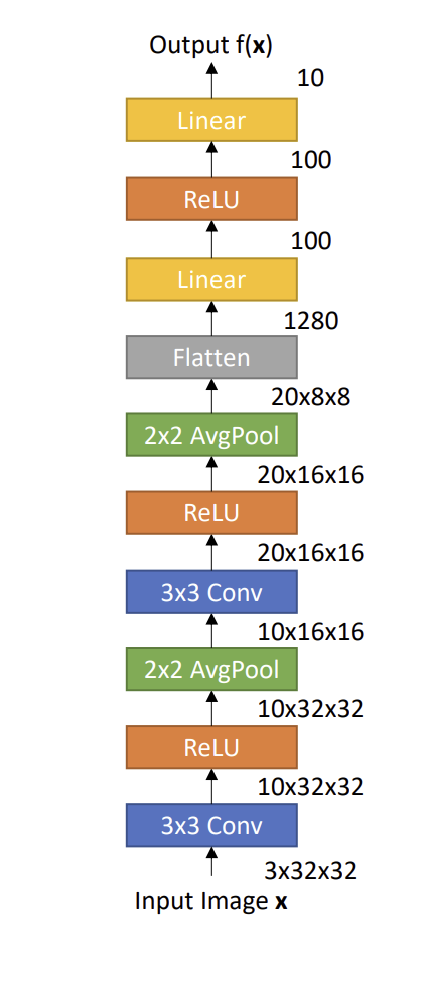
\includegraphics[width=\linewidth]{Images/5.png}
    \end{minipage}

    Download the skeleton code \texttt{hw4.ipynb} from the course website. Complete the skeleton code. In order to get full marks, your report should include:

    \begin{enumerate}
        \item Your code.
        \item Training loss curve.
        \item Test error (overall).
        \item Test error (each class).
    \end{enumerate}

    \textbf{Hint:} You may find the \href{https://pytorch.org/tutorials/beginner/deep_learning_60min_blitz.html}{official PyTorch tutorial} helpful before implementing the network

    \newpage

    \begin{soln}
        Code is attached at the end.
        \begin{center}
            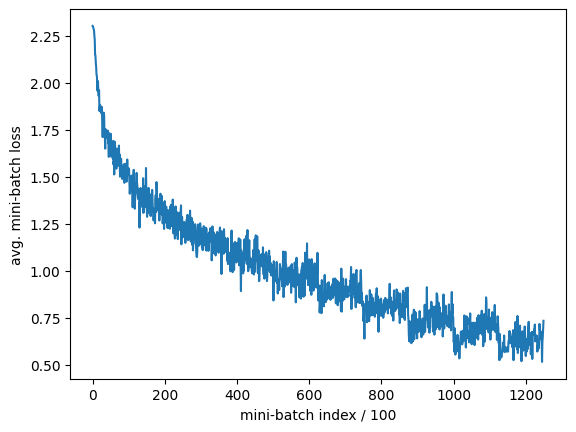
\includegraphics[width=0.4\textwidth]{Images/5_loss.png}
        \end{center}
        My overall test error is 35\%. By class: plane - $25\%$, car - $27\%$, bird - $54\%$, cat - $56\%$, deer - $30\%$, dog - $56\%$, frog - $36\%$, horse - $29\%$, ship - $19\%$, truck - $21\%$.
    \end{soln}
\end{prob}

% --- Problem 6 ---
\begin{prob}[\textbf{(Extra Credit - 15 points) Improve the performance of the CNN on the CIFAR-10 dataset}]
    The problem setting is the same as Problem 5. You can use the same skeleton code \texttt{hw4.ipynb}. Try to modify the architecture of the previous one and improve the performance. You can also make changes other than the architecture such as loss function, data preprocessing, etc. Your report should include:
    
    \begin{enumerate}
        \item Your code.
        \item Training loss curve.
        \item Test error (overall).
        \item Test error (each class).
        \item Your main modification. You're encouraged to provide a detailed description and analysis.
    \end{enumerate}

    \begin{soln}
        Code is attached at the end.
        \begin{center}
            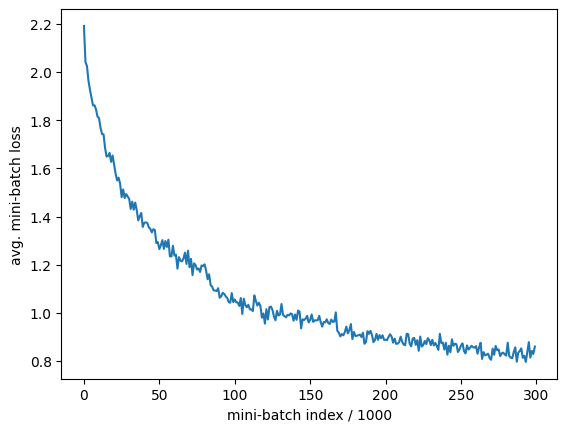
\includegraphics[width=0.4\textwidth]{Images/6_loss.png}
        \end{center}
        After a lot of tinkering, I managed to improve my overall test error to 33\%. By class: plane - $32\%$, car - $22\%$, bird - $49\%$, cat - $51\%$, deer - $36\%$, dog - $46\%$, frog - $27\%$, horse - $34\%$, ship - $22\%$, truck - $25\%$.
        
        To improve on the baseline CNN, I first increased model capacity by adding a third conv block and expanding the channel progression to $3 \to 32 \to 64 \to 128$. I inserted BatchNorm2d after each conv layer to stabilize training and speed up convergence. I also replaced average pooling with max pooling to better preserve strong activations. To reduce overfitting, I introduced dropout layers. Together, these changes raised test accuracy from about 65\% to 67\%, with the largest gains on car, ship, and frog, while cat and bird remained the most difficult classes, as is typical for CIFAR-10.
    \end{soln}
\end{prob}
\end{probset}
\end{document}